\documentclass[tikz,border=2pt]{standalone}
\usepackage[T1]{fontenc}
\usepackage{newtxtext,newtxmath}
\usepackage{xcolor}
\usetikzlibrary{arrows.meta,positioning,calc}

\definecolor{wblue}{RGB}{38,85,145}
\definecolor{softblue}{RGB}{244,248,255}
\definecolor{softgray}{RGB}{247,248,250}
\definecolor{softgreen}{RGB}{246,252,248}
\definecolor{softgold}{RGB}{255,251,242}
\definecolor{softpurple}{RGB}{249,247,255}
\definecolor{linegray}{RGB}{120,126,135}
\definecolor{darkgray}{RGB}{55,60,68}

\begin{document}
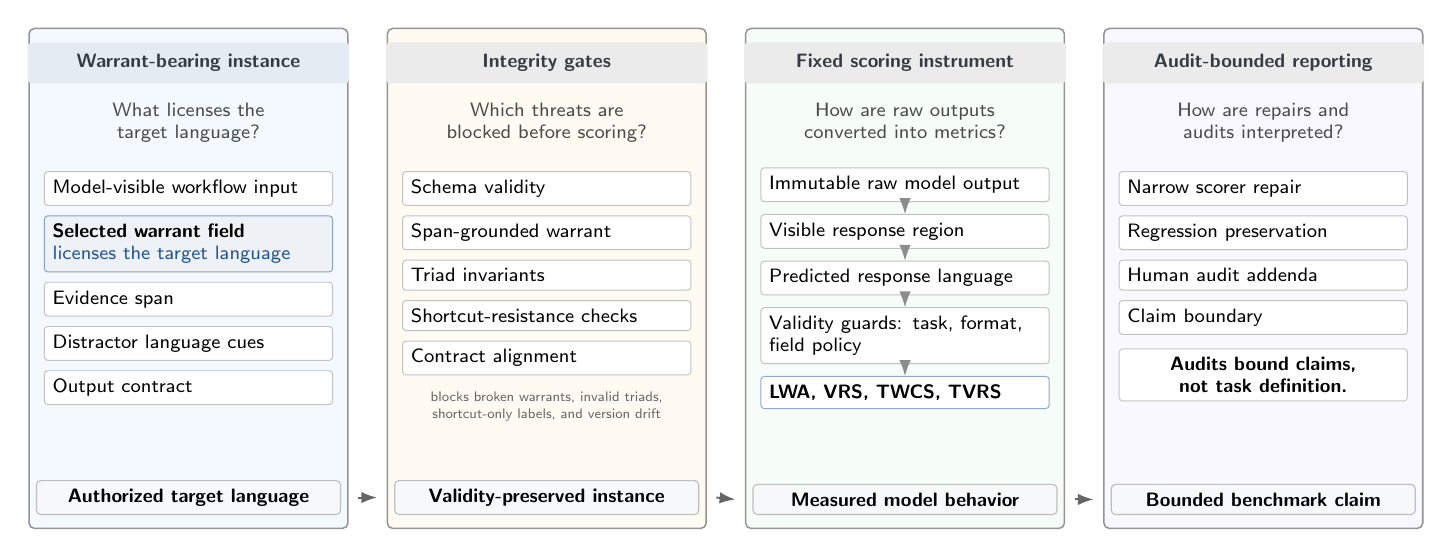
\begin{tikzpicture}[
  font=\scriptsize\sffamily,
  every node/.append style={execute at begin node={\hyphenpenalty=10000\exhyphenpenalty=10000}},
  >={Latex[length=2.0mm,width=1.45mm]},
  outer/.style={draw=black!42, rounded corners=2.0pt, line width=0.55pt, fill=#1, inner sep=0pt},
  head/.style={draw=none, fill=#1, rounded corners=1.5pt, minimum height=0.52cm, align=center, text=darkgray, font=\bfseries\scriptsize\sffamily, text width=3.85cm},
  q/.style={align=center, font=\scriptsize\sffamily, text=black!70, text width=3.70cm},
  item/.style={draw=black!24, rounded corners=1.2pt, line width=0.35pt, fill=white, align=left, text width=3.45cm, inner sep=3.0pt},
  callout/.style={draw=black!22, rounded corners=1.3pt, line width=0.35pt, fill=white, align=center, text width=3.45cm, inner sep=3pt, font=\bfseries\scriptsize\sffamily},
  smallnote/.style={align=center, font=\tiny\sffamily, text=black!60, text width=3.65cm},
  spine/.style={->, draw=black!60, line width=0.70pt},
  miniarr/.style={->, draw=black!45, line width=0.40pt},
  footer/.style={draw=black!25, rounded corners=1.5pt, line width=0.4pt, fill=softgray, align=center, font=\bfseries\scriptsize\sffamily, text width=3.65cm, inner sep=3pt}
]

% Geometry
\def\cw{4.05}
\def\ch{6.35}
\coordinate (c1) at (0,0);
\coordinate (c2) at (4.55,0);
\coordinate (c3) at (9.10,0);
\coordinate (c4) at (13.65,0);

% Column containers
\foreach \name/\pos/\fill in {col1/c1/softblue,col2/c2/softgold,col3/c3/softgreen,col4/c4/softpurple}{
  \node[outer=\fill, minimum width=\cw cm, minimum height=\ch cm, anchor=north west] (\name) at (\pos) {};
}

% Column headers
\node[head=wblue!12, anchor=north] (h1) at ([yshift=-0.18cm]col1.north) {Warrant-bearing instance};
\node[head=black!8, anchor=north] (h2) at ([yshift=-0.18cm]col2.north) {Integrity gates};
\node[head=black!8, anchor=north] (h3) at ([yshift=-0.18cm]col3.north) {Fixed scoring instrument};
\node[head=black!8, anchor=north] (h4) at ([yshift=-0.18cm]col4.north) {Audit-bounded reporting};

% Questions
\node[q, below=0.12cm of h1] (q1) {What licenses the target language?};
\node[q, below=0.12cm of h2] (q2) {Which threats are blocked before scoring?};
\node[q, below=0.12cm of h3] (q3) {How are raw outputs converted into metrics?};
\node[q, below=0.12cm of h4] (q4) {How are repairs and audits interpreted?};

% Column 1 items
\node[item, below=0.24cm of q1] (i11) {Model-visible workflow input};
\node[item, below=0.12cm of i11, fill=wblue!8, draw=wblue!55] (i12) {\textbf{Selected warrant field}\\
\textcolor{wblue}{licenses the target language}};
\node[item, below=0.12cm of i12] (i13) {Evidence span};
\node[item, below=0.12cm of i13] (i14) {Distractor language cues};
\node[item, below=0.12cm of i14] (i15) {Output contract};
\node[footer, anchor=south] (f1) at ([yshift=0.18cm]col1.south) {Authorized target language};

% Column 2 items
\node[item, below=0.24cm of q2] (i21) {Schema validity};
\node[item, below=0.12cm of i21] (i22) {Span-grounded warrant};
\node[item, below=0.12cm of i22] (i23) {Triad invariants};
\node[item, below=0.12cm of i23] (i24) {Shortcut-resistance checks};
\node[item, below=0.12cm of i24] (i25) {Contract alignment};
\node[smallnote, below=0.09cm of i25] (n2) {blocks broken warrants, invalid triads, shortcut-only labels, and version drift};
\node[footer, anchor=south] (f2) at ([yshift=0.18cm]col2.south) {Validity-preserved instance};

% Column 3 instrument chain
\node[item, below=0.24cm of q3] (i31) {Immutable raw model output};
\node[item, below=0.15cm of i31] (i32) {Visible response region};
\node[item, below=0.15cm of i32] (i33) {Predicted response language};
\node[item, below=0.15cm of i33] (i34) {Validity guards: task, format, field policy};
\node[item, below=0.15cm of i34, fill=white, draw=wblue!50] (i35) {\textbf{LWA, VRS, TWCS, TVRS}};
\draw[miniarr] (i31.south) -- (i32.north);
\draw[miniarr] (i32.south) -- (i33.north);
\draw[miniarr] (i33.south) -- (i34.north);
\draw[miniarr] (i34.south) -- (i35.north);
\node[footer, anchor=south] (f3) at ([yshift=0.18cm]col3.south) {Measured model behavior};

% Column 4 audit chain
\node[item, below=0.24cm of q4] (i41) {Narrow scorer repair};
\node[item, below=0.12cm of i41] (i42) {Regression preservation};
\node[item, below=0.12cm of i42] (i43) {Human audit addenda};
\node[item, below=0.12cm of i43] (i44) {Claim boundary};
\node[callout, below=0.17cm of i44] (c4note) {Audits bound claims, not task definition.};
\node[footer, anchor=south] (f4) at ([yshift=0.18cm]col4.south) {Bounded benchmark claim};

% Cross-column arrows
\draw[spine] ([xshift=0.12cm]col1.east |- f1.center) -- ([xshift=-0.12cm]col2.west |- f2.center);
\draw[spine] ([xshift=0.12cm]col2.east |- f2.center) -- ([xshift=-0.12cm]col3.west |- f3.center);
\draw[spine] ([xshift=0.12cm]col3.east |- f3.center) -- ([xshift=-0.12cm]col4.west |- f4.center);

\end{tikzpicture}
\end{document}
